\chapter{Flows}
\section{Assumptions}
We assume that the whole design is synchronous to a single clock, clk\_proc.

logic mux

...

\section{Structure}
Flow connexion is composed by three electric signals :
\begin{itemize}
\item a data bus of the size of one data with \emph{\_data} suffix
\item a data valid signal to indicate that a data is present on the data bus with \emph{\_dv} suffix
\item a flow valid signal to delimit the beginning of the flow and the end with \emph{\_fv} suffix
\end{itemize}

\begin{figure}[h!]
\centering
\begin{tikzpicture}[node distance=8cm]
\tikzset{blocstyle/.style={block,rectangle,minimum height=3cm,minimum width=3.5cm}};

% blocks
\node[blocstyle] (bloc1) {block1};
\node[blocstyle,right of=bloc1] (bloc2) {block2};

% Flow to
\path[connect,->] ([yshift=0.5cm]bloc1.east) -- node[above]{flow1\_data} node{/} ([yshift=0.5cm]bloc2.west);
\path[connect,->] (bloc1.east) -- node[above]{flow1\_dv} (bloc2.west);
\path[connect,->] ([yshift=-0.5cm]bloc1.east) -- node[above]{flow1\_fv} ([yshift=-0.5cm]bloc2.west);

% flow tube
\path[connect,dashed] ([xshift=0.5cm,yshift=1cm]bloc1.east) -- ([xshift=-0.5cm,yshift=1cm]bloc2.west);
\path[connect,dashed] ([xshift=0.5cm,yshift=-1cm]bloc1.east) -- node[below]{flow} ([xshift=-0.5cm,yshift=-1cm]bloc2.west);
\end{tikzpicture}
\caption{Details on flow connexion}
\end{figure}

All theses signals are synchronous on clk\_proc clock.

\section{Timing}
\begin{figure}[h!]
\centering
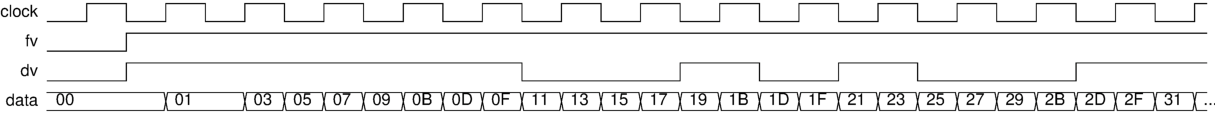
\includegraphics[width=\textwidth]{wave.pdf}
\caption{Example timing for flow signals}
\end{figure}

\section{Clock}
All the flow transmission are synchronous on the same clock, clk\_proc. Like that, we don't need diferent clock domain for data transmission. If a process or IO need to internally work with a different clock, clock syncronisation have to be done internally of the block.

\section{Flow properties}
